\documentclass[12pt,a4paper]{article}
\usepackage{graphicx}
\usepackage{gensymb}
\usepackage{amsmath}
\usepackage{bm}
\usepackage{tikz}
\tikzset{
    node distance=2cm, % specifies the minimum distance between two nodes. Change if necessary.
    }
\title{Case Study Modelling an Electronic Component}
\author{
  Azure Hutchings
  \and
  Jean-Luc Danoy
  \and
  Faris Saad S Alsubaie
}
\date{28 October 2019}
 
\begin{document}
 
\begin{titlepage}
\maketitle
\end{titlepage}

\renewcommand{\abstractname}{Executive Summary}
\begin{abstract}
Write Abstract Here
\end{abstract}

\pagebreak

\tableofcontents

\pagebreak

\section{Introduction}

\subsection{Purpose of the Report}
The following report investigates the steady-state heat distribution in a newly designed component. 

The report will discuss the mathematical model of the heat distribution in the component and the numerical methods used to solve it in MATLAB. 

\subsection{The Maths of the Problem}

\begin{figure}[h!]
	\includegraphics[width=\linewidth]{images/Component.png}
	\caption{Schematic of electronic component.}
	\label{fig:componentSchematic}
\end{figure}

The component schematic is shown in Figure \ref{fig:componentSchematic}. The location of the component within the device means it's subject to different temperature condition along it's boundaries. The boundary A-B is in perfect thermal contact with another component which the temperature is known to 70\degree C. The boundary C-D is also in perfect thermal contact with another component which the temperature is known to be 40\degree C. The boundary A-E-D is thermally insulated and the boundary B-C is exposed to the air at ambient temperature.
\\\\
This type of model can be described with Laplace's equation. Letting $T(x,y)$ represent the temperature of the component at point $(x, y)$, the model is as follows	

\begin{center}
\begin{tabular}{c c}
$\frac{\partial^2 T}{\partial x^2}+\frac{\partial^2 T}{\partial y^2}=0$ & in the interior\\
$T = 70$ & on boundary A-B \\
$T = 40$ & on boundary C-D \\
$\boldsymbol{\nabla} T \cdot {\hat{\textbf{n}}} = 0$ & on boundary A-E-D\\
$k\boldsymbol{\nabla}T\cdot\hat{\textbf{n}} = h(T_{\infty} - T)$ & on boundary B-C
\end{tabular}
\end{center}
Where the thermal conductivity is $k=3Wm^{-1}C^{-1}$, and the heat transfer coefficient is $h=20 Wm^{-2}C^{-1}$. To begin with, we will assume the ambient termperature is $T_\infty = 20$.
\clearpage
\section{Discretising the Problem}
If this was left as a continuous partial differential equation, we would need to analytically solve it. However, it can be much quicker to numerically solve this problem and still retain a high degree of accuracy with the final answers. In this section we will show how we converted the analytical problem to a numerical problem, how the mesh was constructed, the node ordering used, the linear system we dervied from the mesh and discuss the matrix that was created from it.

\subsection{Analytical approach}
To build a numerical approach, we must first understand the basics of the analytical method for solving heat distributions. \\\\The Heat Equation is a partial differential equation which states that the change in temperature over time is proportional to the double derivative of temperature with repsect to its spacial variables
\begin{center}
$\frac{\partial u}{\partial t} \propto \bigg(\frac{\partial^2 u}{\partial x^2} + \frac{\partial^2 u}{\partial y^2}\bigg)$
\\
$\frac{\partial u}{\partial t} = D\bigg{(}\frac{\partial^2 u}{\partial x^2} + \frac{\partial^2 u}{\partial y^2}\bigg{)}$
\end{center}

\subsection{Numerical approach}
Suppose we had a function $\phi(x,y,t)$ which gives the temperature at the point (x,y) on a 2-dimensional plane where t is the time since the start of the initial conditions. If the function has a steady-state solution, then it means at some point in time, any increase in time will not result in a change of temperature. This means that 
\begin{center}
$\frac{d\phi}{dx}|_{x_i}\approx\frac{\phi(x_i+\Delta x)-\phi(x_i)}{\Delta x}$,
\end{center}
where the change in $x$ along $\phi$ at the point $x_i$ is approximately the functions forward difference over the distance between nodes. We can then take the derivative of this again using backwards difference to get the second derivative centered around $x_i$.
\begin{center}
$\frac{d^2\phi}{dx^2}|_{x_i}\approx\frac{\phi(x_i+\Delta x)-2\phi(x_i)+\phi(x_i-\Delta x)}{(\Delta x)^2}$,
\end{center}
To numerically solve this problem, we must construct a finite difference mesh and create a matrix to represent this information.\\\\
By splitting the component up into intervals of 0.01, we can split the component into a 7x7 grid. Given the previous mesh
\subsection*{Finite Difference Mesh}
There are 3 different types of mesh that need to be created. These are for the A-E-D boundary, the inside of the mesh, and on the B-C boundary.\\\\On the interior of the mesh, each node contains 4 other nodes adjacent to it, and the change in temperature at that node is given by the equation
\begin{center}
$\frac{\partial^2 T}{\partial x^2}+\frac{\partial^2 T}{\partial y^2}=0$
\\
$\frac{\partial}{\partial x}(\frac{\partial T}{\partial x}) + \frac{\partial}{\partial x}(\frac{\partial T}{\partial y}) = 0$
\\
$\frac{\partial T}{\partial x}=\frac{T_{i+1}-T_i}{\delta}$ 
\end{center}
\begin{center}
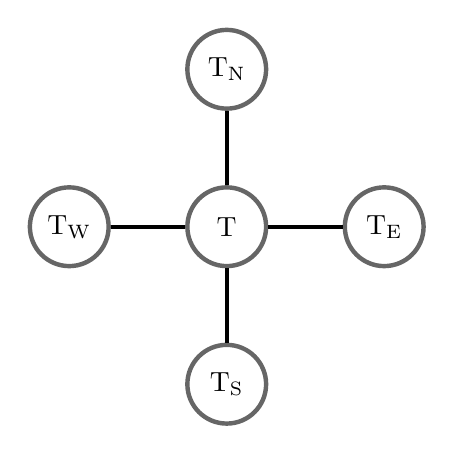
\begin{tikzpicture}[
roundnode/.style={circle, draw=black!60, ultra thick,  minimum size=10mm},
]
\node[roundnode] (center) {T};
\node[roundnode] (left) [left of=center] {T$_\text{W}$};
\node[roundnode] (right) [right of=center] {T$_\text{E}$};
\node[roundnode] (above) [above of=center] {T$_\text{N}$};
\node[roundnode] (below) [below of=center] {T$_\text{S}$};

\draw[ultra thick,-] (left.east) -- (center.west);
\draw[ultra thick,-] (above.south) -- (center.north);
\draw[ultra thick,-] (right.west) -- (center.east);
\draw[ultra thick,-] (below.north) -- (center.south);
\end{tikzpicture}
\end{center}
%\subsection{Research methods}
%
%
%\subsection{Limitations and assumptions}
%
%\section{Discussion}
%
%\subsection{Method}
%
%\subsubsection{Procedures}
%
%\subsubsection{Sample Size}
%
%\subsubsection{Selection Criteria}
%
%\subsection{Discussion and analysis of data}
%
%\subsubsection{Issue 1}
%
%\subsubsection{Issue 2}
%
%\subsubsection{Issue 3}
%
%\subsubsection{Reliability and accuracy of data}
%
%\section{Conclusions}
%
%\section{Recommendations}
%
%\subsection{Recommendation 1}
%
%\subsection{Recommendation 2}
%
%\section{References}
%
%\section{Appendices}
 
\end{document}